\documentclass[11pt,ignorenonframetext,]{beamer}
\setbeamertemplate{caption}[numbered]
\setbeamertemplate{caption label separator}{: }
\setbeamercolor{caption name}{fg=normal text.fg}
\beamertemplatenavigationsymbolsempty
\usepackage{lmodern}
\usepackage{amssymb,amsmath}
\usepackage{ifxetex,ifluatex}
\usepackage{fixltx2e} % provides \textsubscript
\ifnum 0\ifxetex 1\fi\ifluatex 1\fi=0 % if pdftex
  \usepackage[T1]{fontenc}
  \usepackage[utf8]{inputenc}
\else % if luatex or xelatex
  \ifxetex
    \usepackage{mathspec}
  \else
    \usepackage{fontspec}
  \fi
  \defaultfontfeatures{Ligatures=TeX,Scale=MatchLowercase}
\fi
\usetheme[]{metropolis}
% use upquote if available, for straight quotes in verbatim environments
\IfFileExists{upquote.sty}{\usepackage{upquote}}{}
% use microtype if available
\IfFileExists{microtype.sty}{%
\usepackage{microtype}
\UseMicrotypeSet[protrusion]{basicmath} % disable protrusion for tt fonts
}{}
\newif\ifbibliography
\hypersetup{
            pdftitle={Lecture 16},
            pdfauthor={Colin Rundel},
            pdfborder={0 0 0},
            breaklinks=true}
\urlstyle{same}  % don't use monospace font for urls
\usepackage{color}
\usepackage{fancyvrb}
\newcommand{\VerbBar}{|}
\newcommand{\VERB}{\Verb[commandchars=\\\{\}]}
\DefineVerbatimEnvironment{Highlighting}{Verbatim}{commandchars=\\\{\}}
% Add ',fontsize=\small' for more characters per line
\newenvironment{Shaded}{}{}
\newcommand{\KeywordTok}[1]{\textcolor[rgb]{0.00,0.44,0.13}{\textbf{#1}}}
\newcommand{\DataTypeTok}[1]{\textcolor[rgb]{0.56,0.13,0.00}{#1}}
\newcommand{\DecValTok}[1]{\textcolor[rgb]{0.25,0.63,0.44}{#1}}
\newcommand{\BaseNTok}[1]{\textcolor[rgb]{0.25,0.63,0.44}{#1}}
\newcommand{\FloatTok}[1]{\textcolor[rgb]{0.25,0.63,0.44}{#1}}
\newcommand{\ConstantTok}[1]{\textcolor[rgb]{0.53,0.00,0.00}{#1}}
\newcommand{\CharTok}[1]{\textcolor[rgb]{0.25,0.44,0.63}{#1}}
\newcommand{\SpecialCharTok}[1]{\textcolor[rgb]{0.25,0.44,0.63}{#1}}
\newcommand{\StringTok}[1]{\textcolor[rgb]{0.25,0.44,0.63}{#1}}
\newcommand{\VerbatimStringTok}[1]{\textcolor[rgb]{0.25,0.44,0.63}{#1}}
\newcommand{\SpecialStringTok}[1]{\textcolor[rgb]{0.73,0.40,0.53}{#1}}
\newcommand{\ImportTok}[1]{#1}
\newcommand{\CommentTok}[1]{\textcolor[rgb]{0.38,0.63,0.69}{\textit{#1}}}
\newcommand{\DocumentationTok}[1]{\textcolor[rgb]{0.73,0.13,0.13}{\textit{#1}}}
\newcommand{\AnnotationTok}[1]{\textcolor[rgb]{0.38,0.63,0.69}{\textbf{\textit{#1}}}}
\newcommand{\CommentVarTok}[1]{\textcolor[rgb]{0.38,0.63,0.69}{\textbf{\textit{#1}}}}
\newcommand{\OtherTok}[1]{\textcolor[rgb]{0.00,0.44,0.13}{#1}}
\newcommand{\FunctionTok}[1]{\textcolor[rgb]{0.02,0.16,0.49}{#1}}
\newcommand{\VariableTok}[1]{\textcolor[rgb]{0.10,0.09,0.49}{#1}}
\newcommand{\ControlFlowTok}[1]{\textcolor[rgb]{0.00,0.44,0.13}{\textbf{#1}}}
\newcommand{\OperatorTok}[1]{\textcolor[rgb]{0.40,0.40,0.40}{#1}}
\newcommand{\BuiltInTok}[1]{#1}
\newcommand{\ExtensionTok}[1]{#1}
\newcommand{\PreprocessorTok}[1]{\textcolor[rgb]{0.74,0.48,0.00}{#1}}
\newcommand{\AttributeTok}[1]{\textcolor[rgb]{0.49,0.56,0.16}{#1}}
\newcommand{\RegionMarkerTok}[1]{#1}
\newcommand{\InformationTok}[1]{\textcolor[rgb]{0.38,0.63,0.69}{\textbf{\textit{#1}}}}
\newcommand{\WarningTok}[1]{\textcolor[rgb]{0.38,0.63,0.69}{\textbf{\textit{#1}}}}
\newcommand{\AlertTok}[1]{\textcolor[rgb]{1.00,0.00,0.00}{\textbf{#1}}}
\newcommand{\ErrorTok}[1]{\textcolor[rgb]{1.00,0.00,0.00}{\textbf{#1}}}
\newcommand{\NormalTok}[1]{#1}
\usepackage{graphicx,grffile}
\makeatletter
\def\maxwidth{\ifdim\Gin@nat@width>\linewidth\linewidth\else\Gin@nat@width\fi}
\def\maxheight{\ifdim\Gin@nat@height>\textheight0.8\textheight\else\Gin@nat@height\fi}
\makeatother
% Scale images if necessary, so that they will not overflow the page
% margins by default, and it is still possible to overwrite the defaults
% using explicit options in \includegraphics[width, height, ...]{}
\setkeys{Gin}{width=\maxwidth,height=\maxheight,keepaspectratio}

% Prevent slide breaks in the middle of a paragraph:
\widowpenalties 1 10000
\raggedbottom

\AtBeginPart{
  \let\insertpartnumber\relax
  \let\partname\relax
  \frame{\partpage}
}
\AtBeginSection{
  \ifbibliography
  \else
    \let\insertsectionnumber\relax
    \let\sectionname\relax
    \frame{\sectionpage}
  \fi
}
\AtBeginSubsection{
  \let\insertsubsectionnumber\relax
  \let\subsectionname\relax
  \frame{\subsectionpage}
}

\usepackage[normalem]{ulem}
% avoid problems with \sout in headers with hyperref:
\pdfstringdefDisableCommands{\renewcommand{\sout}{}}
\setlength{\parindent}{0pt}
\setlength{\parskip}{6pt plus 2pt minus 1pt}
\setlength{\emergencystretch}{3em}  % prevent overfull lines
\providecommand{\tightlist}{%
  \setlength{\itemsep}{0pt}\setlength{\parskip}{0pt}}
\setcounter{secnumdepth}{0}

\usepackage{geometry}
\usepackage{graphicx}
\usepackage{amssymb}
\usepackage{color}          	% gives color options
\usepackage{url}		% produces hyperlinks
\usepackage[english]{babel}
\usepackage{colortbl}	% allows for color usage in tables
\usepackage{multirow}	% allows for rows that span multiple rows in tables
\usepackage{xcolor}		% this package has a variety of color options
\usepackage{calc}
\usepackage{multicol}
\usepackage{wrapfig}
\usepackage{textcomp}
\usepackage{bm}
\usepackage{bbm}
\usepackage{setspace}
\usepackage{changepage}
\singlespacing

%%%%%%%%%%%%%%%%
% Small code output
%%%%%%%%%%%%%%%%

%% change fontsize of R code

\makeatletter
\@ifundefined{Shaded}{\newenvironment{Shaded}{}{}}{}
\makeatother


\let\oldShaded\Shaded
\let\endoldShaded\endShaded
\renewenvironment{Shaded}{\footnotesize\begin{spacing}{0.9}\oldShaded}{\endoldShaded\end{spacing}}

%% change fontsize of output
\let\oldverbatim\verbatim
\let\endoldverbatim\endverbatim
\renewenvironment{verbatim}{\footnotesize\begin{spacing}{0.9}\oldverbatim}{\endoldverbatim\end{spacing}}


\newcommand{\tinyoutput}{
  \renewenvironment{Shaded}{\tiny\begin{spacing}{0.9}\oldShaded}{\endoldShaded\end{spacing}}
  \renewenvironment{verbatim}{\tiny\begin{spacing}{0.9}\oldverbatim}{\endoldverbatim\end{spacing}}
}

\newcommand{\scriptoutput}{
  \renewenvironment{Shaded}{\scriptsize\begin{spacing}{0.9}\oldShaded}{\endoldShaded\end{spacing}}
  \renewenvironment{verbatim}{\scriptsize\begin{spacing}{0.9}\oldverbatim}{\endoldverbatim\end{spacing}}
}

\newcommand{\footnoteoutput}{
  \renewenvironment{Shaded}{\footnotesize\begin{spacing}{0.9}\oldShaded}{\endoldShaded\end{spacing}}
  \renewenvironment{verbatim}{\footnotesize\begin{spacing}{0.9}\oldverbatim}{\endoldverbatim\end{spacing}}
}

%\newcommand{\verbatimfont}[1]{\renewcommand{\verbatim@font}{\ttfamily#1}}


%%%%%%%%%%%%%%%%
% Custom Colors
%%%%%%%%%%%%%%%%

\xdefinecolor{oiBlue}{rgb}{0.15, 0.35, 0.55}
\xdefinecolor{gray}{rgb}{0.5, 0.5, 0.5}
\xdefinecolor{darkGray}{rgb}{0.3, 0.3, 0.3}
\xdefinecolor{darkerGray}{rgb}{0.2, 0.2, 0.2}
\xdefinecolor{rubineRed}{rgb}{0.89,0,0.30}
\xdefinecolor{linkCol}{rgb}{0.11,0.49,0.95}	
\xdefinecolor{irishGreen}{rgb}{0,0.60,0}	
\xdefinecolor{darkturquoise}{rgb}{0.44, 0.58, 0.86}
\definecolor{lightGreen}{rgb}{0.533,0.765,0.42}
%\xdefinecolor{hlblue}{rgb}{0.051,0.65,1}
\xdefinecolor{hlblue}{rgb}{ 0.055, 0.639, 0.831}
\definecolor{light}{rgb}{.337,.608,.741}
\definecolor{dark}{rgb}{.337,.608,.741}

\definecolor{cpink}{rgb}{0.93, 0.23, 0.51}

%%%%%%%%%%%%%%%%
% Custom Commands
%%%%%%%%%%%%%%%%

% text colors
\newcommand{\red}[1]{\textit{\textcolor{rubineRed}{#1}}}
\newcommand{\orange}[1]{\textit{\textcolor{orange}{#1}}}
\newcommand{\pink}[1]{\textit{\textcolor{rubineRed!90!white!50}{#1}}}
\newcommand{\green}[1]{\textit{\textcolor{irishGreen}{#1}}}
\newcommand{\blue}[1]{\textit{\textcolor{darkturquoise}{#1}}}
\newcommand{\light}[1]{\textcolor{light}{\textbf{#1}}}
\newcommand{\dark}[1]{\textcolor{dark}{#1}}
\newcommand{\gray}[1]{\textcolor{gray}{#1}}


% links: webURL, webLin, appLink
\newcommand{\webURL}[1]{\urlstyle{same}{\textit{\textcolor{linkCol}{\url{#1}}} }}
\newcommand{\webLink}[2]{\href{#1}{\textcolor{linkCol}{{#2}}}}
\newcommand{\appLink}[2]{\href{#1}{\textcolor{lightGreen!80!black!90}{{#2}}}}

% mail
\newcommand{\mail}[1]{\href{mailto:#1}{\textit{\textcolor{linkCol}{#1}}}}

% highlighting: hl, hlGr, mathhl
\newcommand{\hl}[1]{\textit{\textcolor{hlblue}{#1}}}
\newcommand{\hlGr}[1]{\textit{\textcolor{lightGreen}{#1}}}
\newcommand{\hlRd}[1]{\textit{\textcolor{rubineRed}{#1}}}
\newcommand{\mathhl}[1]{\textcolor{hlblue}{\ensuremath{#1}}}

% example
\newcommand{\ex}[1]{\textcolor{blue}{{{\small (#1)}}}}


\DeclareMathOperator*{\argmin}{arg\,min}
\DeclareMathOperator*{\argmax}{arg\,max}

\title{Lecture 16}
\subtitle{Spatial Data and Cartography}
\author{Colin Rundel}
\date{03/20/2017}

\begin{document}
\frame{\titlepage}

\section{Background}\label{background}

\begin{frame}[fragile]{Analysis of geospatial data in R}

R has a rich package ecosystem for read/writing, manipulating, and
analyzing geospatial data.

Some core packages:

\begin{itemize}
\item
  \texttt{sp} - core classes for handling spatial data, additional
  utility functions.
\item
  \texttt{rgdal} - R interface to \texttt{gdal} (Geospatial Data
  Abstraction Library) for reading and writing spatial data.
\item
  \texttt{rgeos} - R interface to \texttt{geos} (Geometry Engine Open
  Source) library for querying and manipulating spatial data. Reading
  and writing WKT.
\item
  \texttt{raster} - classes and tools for handling spatial raster data.
\end{itemize}

See more -
\href{http://cran.r-project.org/web/views/Spatial.html}{Spatial task
view}

\end{frame}

\begin{frame}[fragile]{Analysis of geospatial data in R}

R has a rich package ecosystem for read/writing, manipulating, and
analyzing geospatial data.

Some core packages:

\begin{itemize}
\item
  \sout{\texttt{sp} - core classes for handling spatial data, additional
  utility functions.}
\item
  \sout{\texttt{rgdal} - R interface to \texttt{gdal} (Geospatial Data
  Abstraction Library) for reading and writing spatial data.}
\item
  \sout{\texttt{rgeos} - R interface to \texttt{geos} (Geometry Engine
  Open Source) library for querying and manipulating spatial data.
  Reading and writing WKT.}
\item
  \texttt{sf} - Combines the functionality of \texttt{sp},
  \texttt{rgdal}, and \texttt{rgeos} into a single package based on tidy
  priciples.
\item
  \texttt{raster} - classes and tools for handling spatial raster data.
\end{itemize}

See more -
\href{http://cran.r-project.org/web/views/Spatial.html}{Spatial task
view}

\end{frame}

\begin{frame}[fragile]{Installing \texttt{sf}}

\footnotesize

The \texttt{sf} package is currently under active development and is
evolving rapidly. The version on CRAN should be reasonably up to date,
but the most current version is always available from
\href{https://github.com/edzer/sfr/}{github}.

Difficulty comes from requirements for external libraries
(\texttt{geos}, \texttt{gdal}, and \texttt{proj4}).

\begin{itemize}
\item
  \emph{Windows} - installing from source works when Rtools is installed
  (system requirements are downloaded from rwinlib)
\item
  \emph{MacOS} - install dependencies via homebrew:
\end{itemize}

\scriptoutput

\begin{verbatim}
brew tap osgeo/osgeo4mac && brew tap --repair
brew install proj 
brew install geos 
brew install udunits
brew unlink gdal
brew install gdal2 
\end{verbatim}

\begin{itemize}
\tightlist
\item
  \emph{Linux} - Install development pacakages for GDAL (\textgreater{}=
  2.0.0), GEOS (\textgreater{}= 3.3.0) and Proj.4 (\textgreater{}=
  4.8.0) from your package manager of choice.
\end{itemize}

\end{frame}

\begin{frame}{Simple Features}

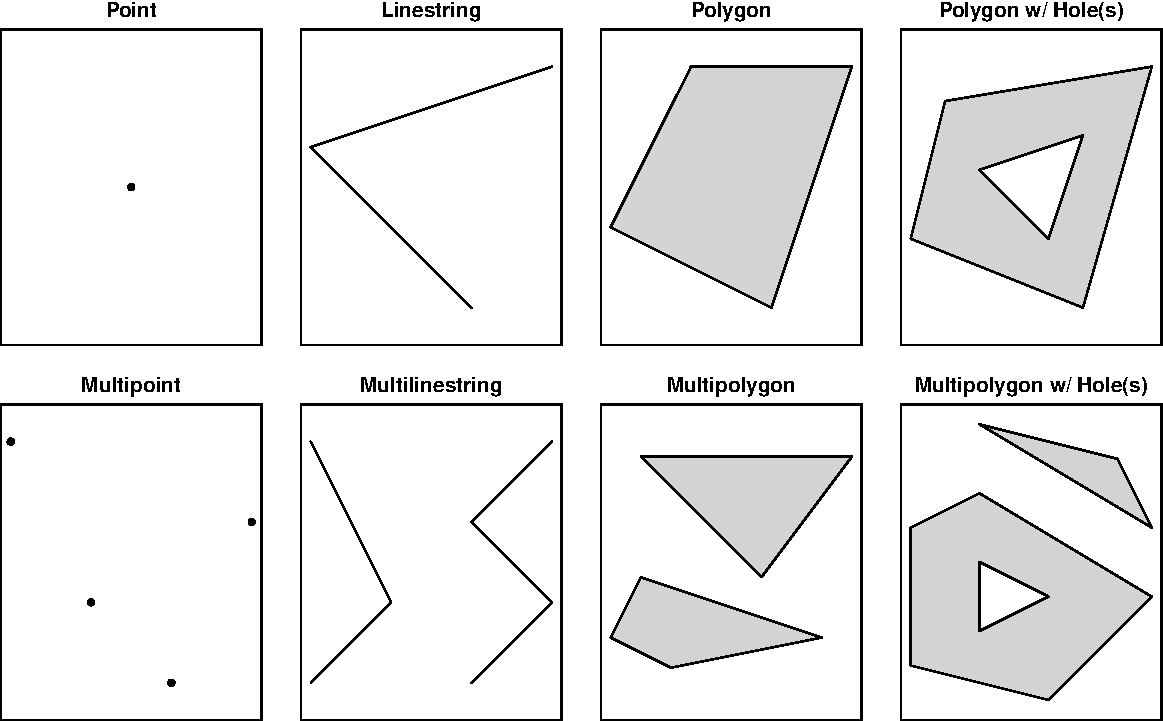
\includegraphics{Lec16_files/figure-beamer/unnamed-chunk-1-1.pdf}

\end{frame}

\begin{frame}{Geometry Collection}

\begin{center}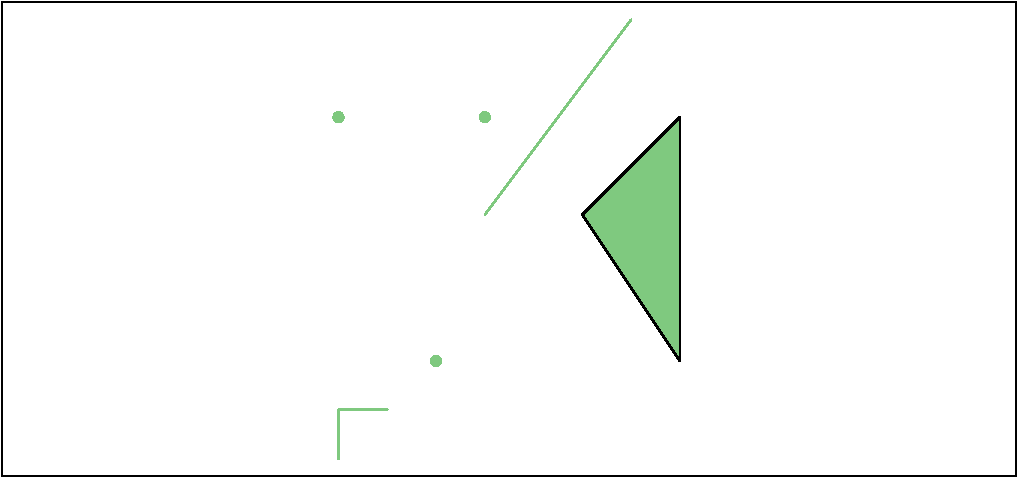
\includegraphics{Lec16_files/figure-beamer/unnamed-chunk-2-1} \end{center}

Point, Multipoint, Multilinestring, Polygon

\end{frame}

\begin{frame}[fragile]{Reading and writing geospatial data via
\texttt{sp}}

\begin{itemize}
\tightlist
\item
  \texttt{maptools}

  \begin{itemize}
  \tightlist
  \item
    \texttt{readShapePoints} / \texttt{writeShapePoints} - Shapefile w/
    points
  \item
    \texttt{readShapeLines} / \texttt{writeShapeLines} - Shapefile w/
    lines
  \item
    \texttt{readShapePoly} / \texttt{writeShapePoly} - Shapefile w/
    polygons
  \item
    \texttt{readShapeSpatial} / \texttt{writeShapeSpatial} - Shapefile
  \end{itemize}
\item
  \texttt{rgdal}

  \begin{itemize}
  \tightlist
  \item
    \texttt{readOGR} / \texttt{writeOGR} - Shapefile, GeoJSON, KML,
    \ldots{}
  \end{itemize}
\item
  \texttt{rgeos}

  \begin{itemize}
  \tightlist
  \item
    \texttt{readWKT} / \texttt{writeWKT} - Well Known Text
  \end{itemize}
\item
  \texttt{sf}

  \begin{itemize}
  \tightlist
  \item
    \texttt{st\_read} / \texttt{st\_write} - Shapefile, GeoJSON, KML,
    \ldots{}
  \end{itemize}
\end{itemize}

\end{frame}

\begin{frame}[fragile]{Reading and writing geospatial data via
\texttt{sp}}

\begin{itemize}
\tightlist
\item
  \sout{\texttt{maptools}}

  \begin{itemize}
  \tightlist
  \item
    \sout{\texttt{readShapePoints} / \texttt{writeShapePoints} -
    Shapefile w/ points}
  \item
    \sout{\texttt{readShapeLines} / \texttt{writeShapeLines} - Shapefile
    w/ lines}
  \item
    \sout{\texttt{readShapePoly} / \texttt{writeShapePoly} - Shapefile
    w/ polygons}
  \item
    \sout{\texttt{readShapeSpatial} / \texttt{writeShapeSpatial} -
    Shapefile}
  \end{itemize}
\item
  \sout{\texttt{rgdal}}

  \begin{itemize}
  \tightlist
  \item
    \sout{\texttt{readOGR} / \texttt{writeOGR} - Shapefile, GeoJSON,
    KML, \ldots{}}
  \end{itemize}
\item
  \texttt{rgeos}

  \begin{itemize}
  \tightlist
  \item
    \texttt{readWKT} / \texttt{writeWKT} - Well Known Text
  \end{itemize}
\item
  \texttt{sf}

  \begin{itemize}
  \tightlist
  \item
    \texttt{st\_read} / \texttt{st\_write} - Shapefile, GeoJSON, KML,
    \ldots{}
  \end{itemize}
\end{itemize}

\end{frame}

\section{Geospatial stuff is
complicated}\label{geospatial-stuff-is-complicated}

\begin{frame}{Projections}

\begin{center}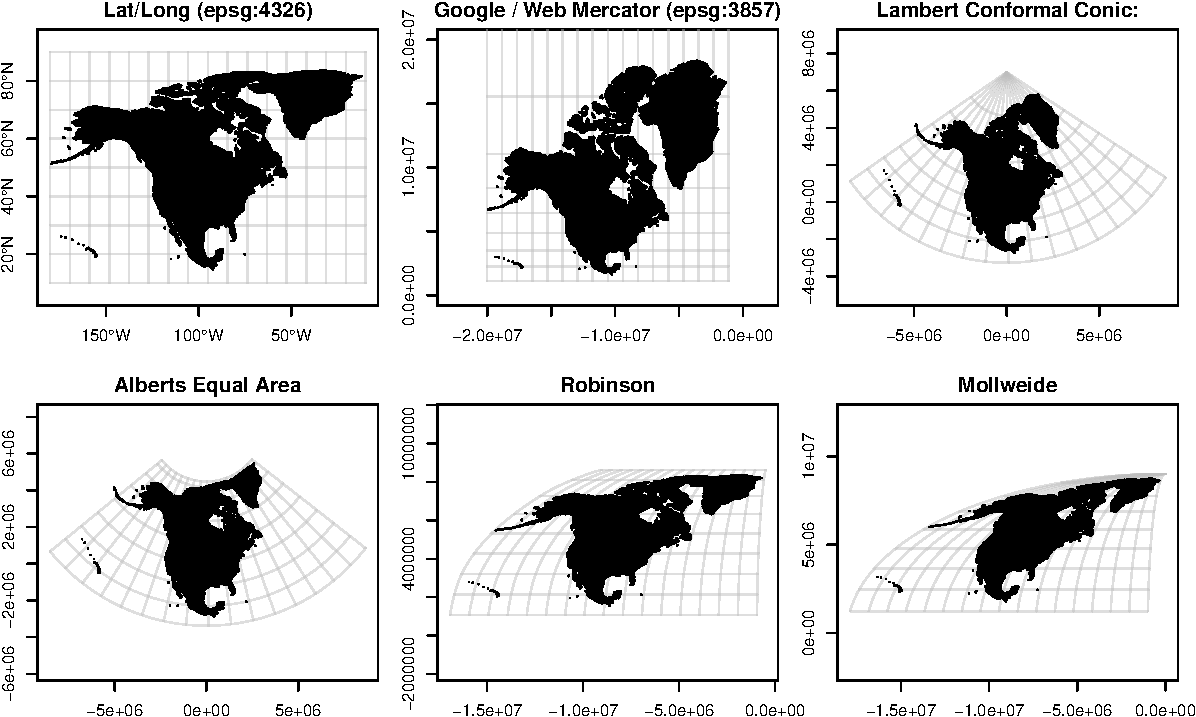
\includegraphics{Lec16_files/figure-beamer/unnamed-chunk-4-1} \end{center}

\end{frame}

\begin{frame}{Dateline}

Want to fly from the Western most point in the US to the Eastern most
point?

\begin{center}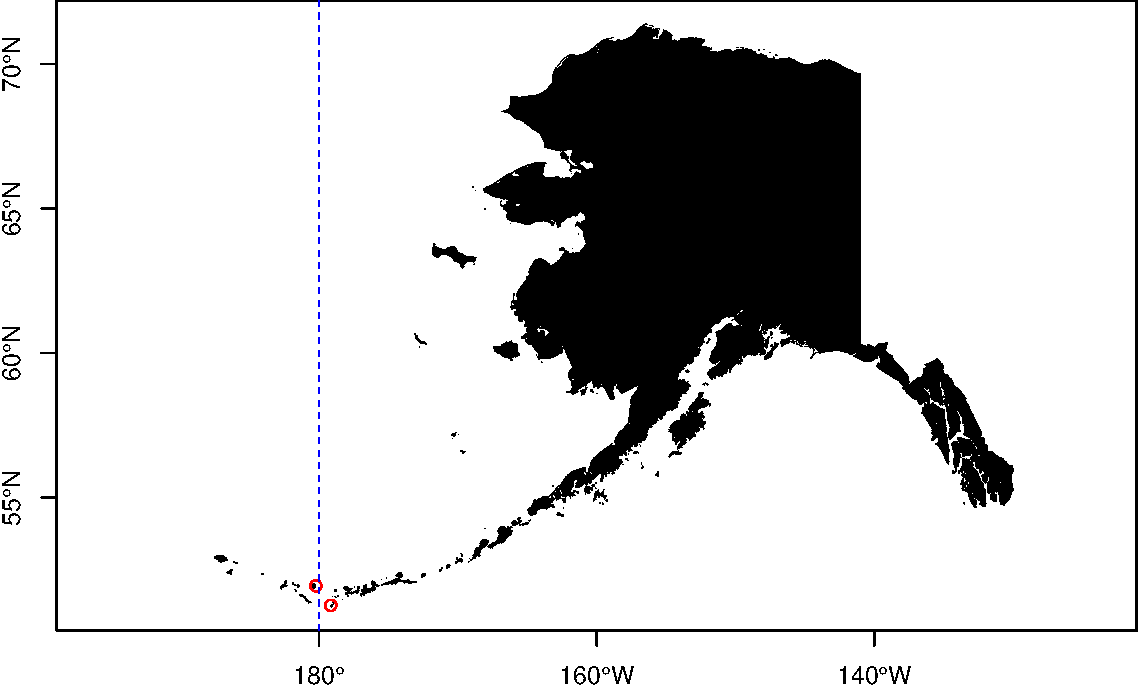
\includegraphics{Lec16_files/figure-beamer/unnamed-chunk-5-1} \end{center}

\end{frame}

\begin{frame}{}

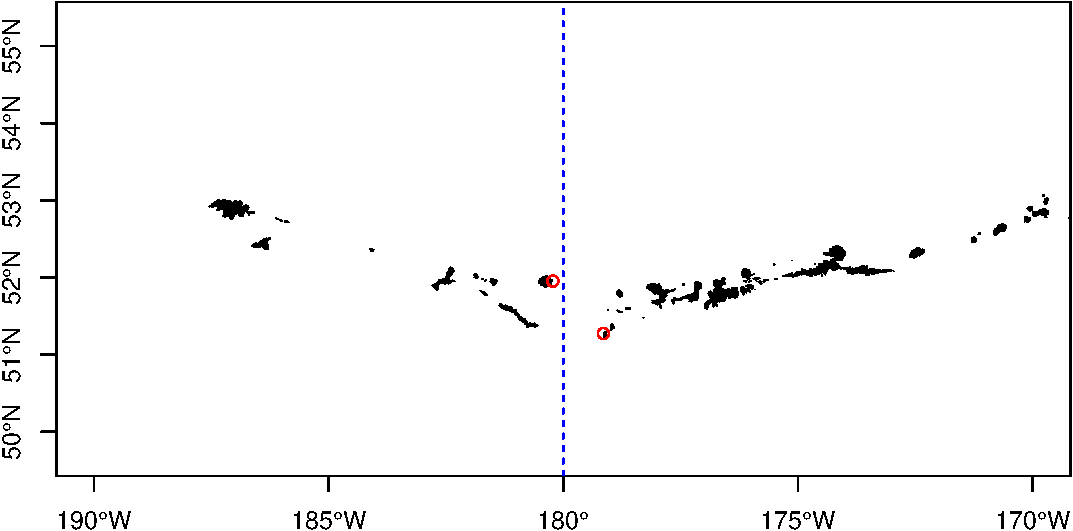
\includegraphics{Lec16_files/figure-beamer/unnamed-chunk-6-1.pdf}

\end{frame}

\begin{frame}{}

\begin{center}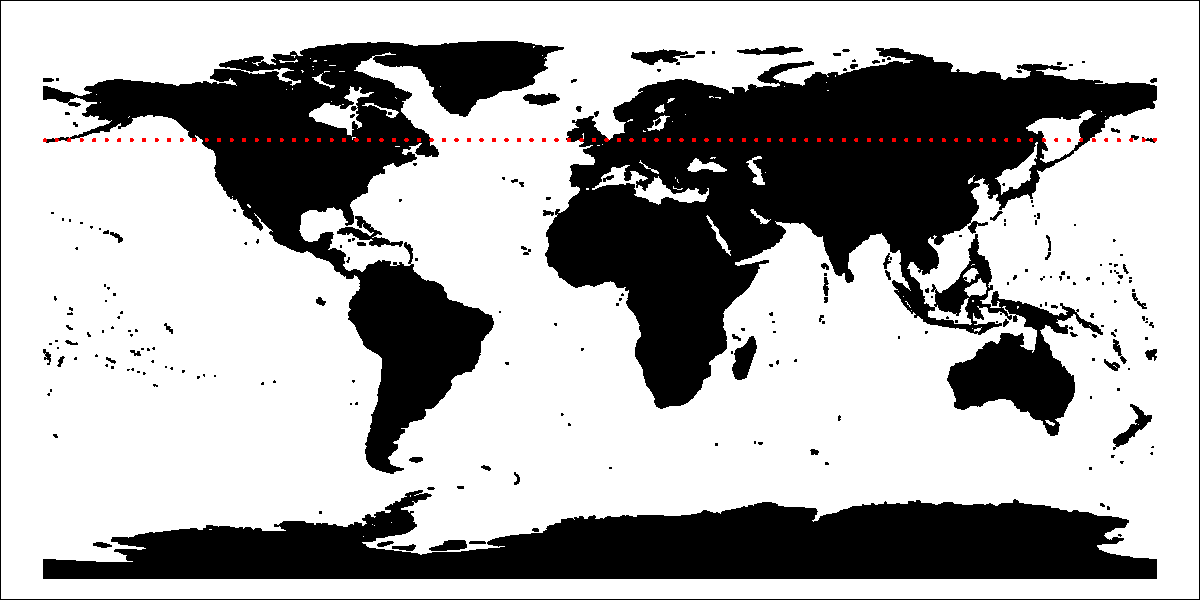
\includegraphics{Lec16_files/figure-beamer/unnamed-chunk-7-1} \end{center}

\end{frame}

\begin{frame}{Relationships}

\begin{center}
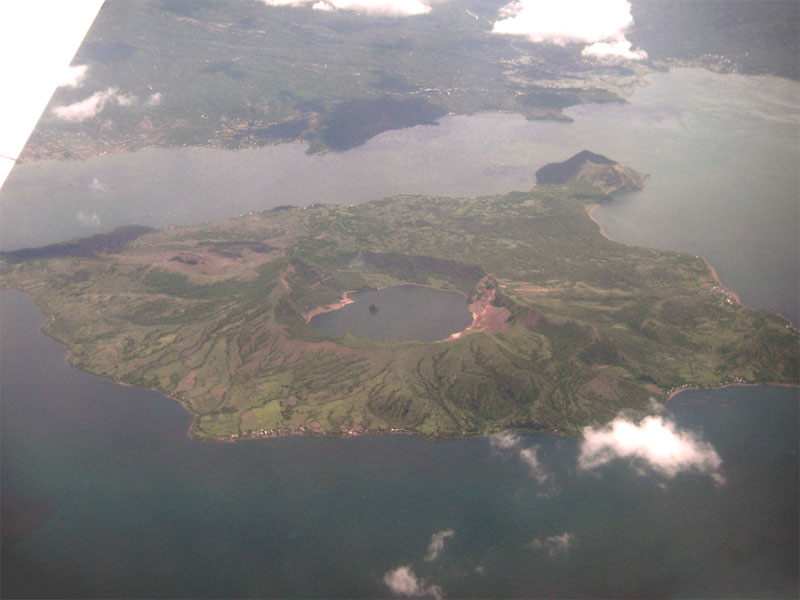
\includegraphics[width=0.6\textwidth]{figs/Taal.png} \\
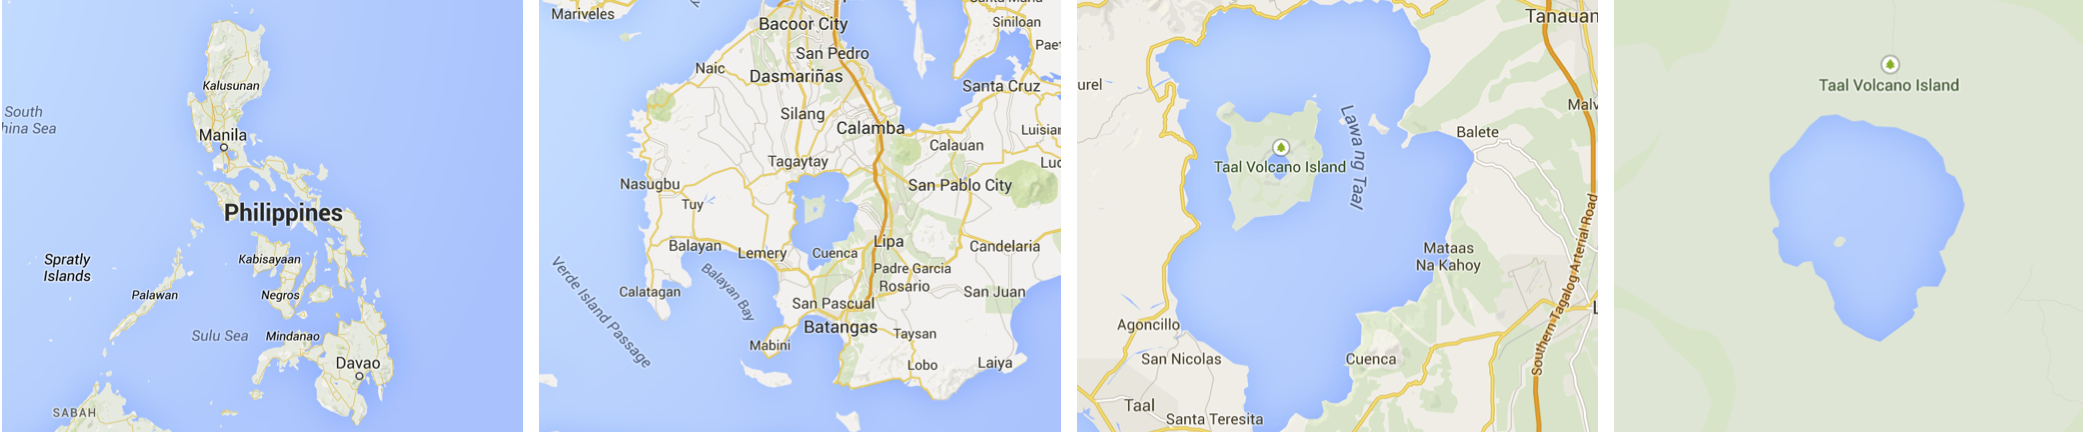
\includegraphics[width=\textwidth]{figs/taal_seq.png}
\end{center}

\end{frame}

\begin{frame}{Distance on a Sphere}

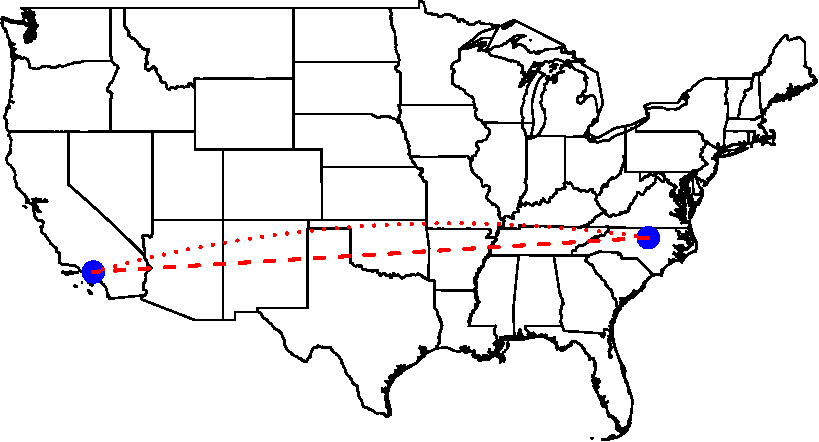
\includegraphics{Lec16_files/figure-beamer/unnamed-chunk-8-1.pdf}

\end{frame}

\begin{frame}{Distance for Simple Features}

\begin{center}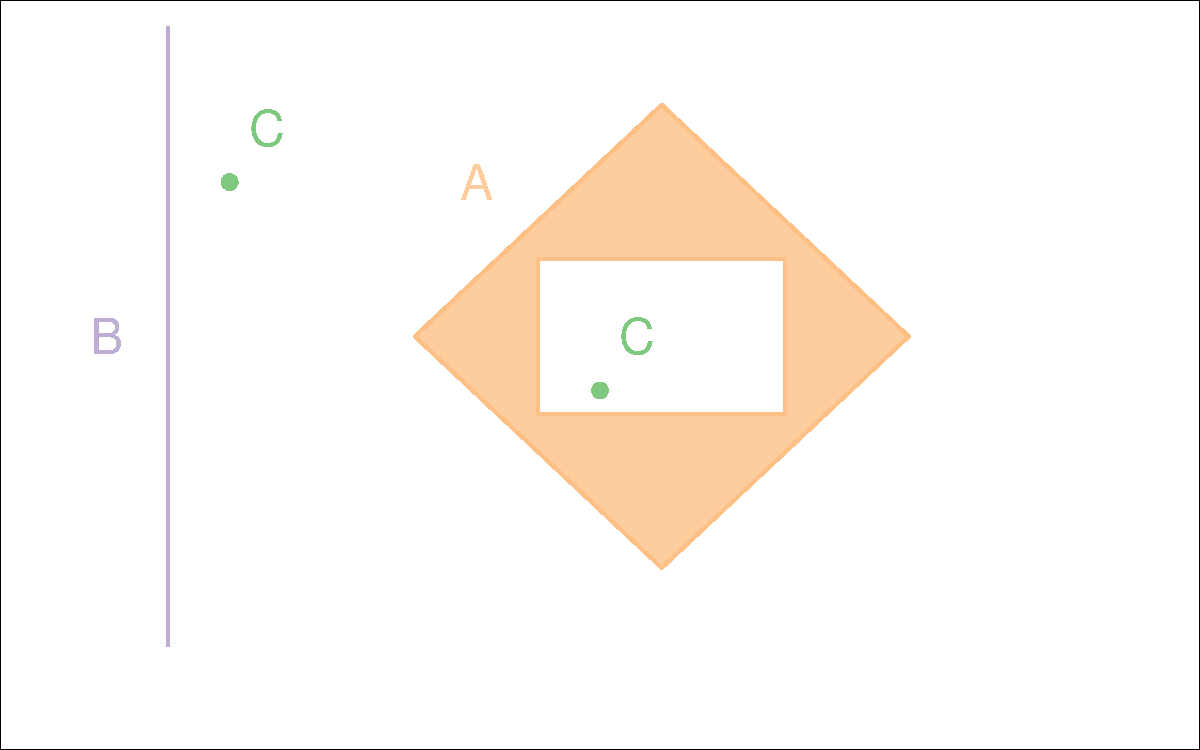
\includegraphics{Lec16_files/figure-beamer/unnamed-chunk-9-1} \end{center}

How do we define the distance between A and B, A and C, or B and C?

\end{frame}

\section{\texorpdfstring{Using \texttt{sf}}{Using sf}}\label{using-sf}

\begin{frame}[fragile]{Example data}

\scriptoutput

\begin{Shaded}
\begin{Highlighting}[]
\NormalTok{nc  =}\StringTok{ }\KeywordTok{st_read}\NormalTok{(}\StringTok{"data/gis/nc_counties/"}\NormalTok{, }\DataTypeTok{quiet=}\OtherTok{TRUE}\NormalTok{, }\DataTypeTok{stringsAsFactors=}\OtherTok{FALSE}\NormalTok{)}
\NormalTok{air =}\StringTok{ }\KeywordTok{st_read}\NormalTok{(}\StringTok{"data/gis/airports/"}\NormalTok{, }\DataTypeTok{quiet=}\OtherTok{TRUE}\NormalTok{, }\DataTypeTok{stringsAsFactors=}\OtherTok{FALSE}\NormalTok{)}
\NormalTok{hwy =}\StringTok{ }\KeywordTok{st_read}\NormalTok{(}\StringTok{"data/gis/us_interstates/"}\NormalTok{, }\DataTypeTok{quiet=}\OtherTok{TRUE}\NormalTok{, }\DataTypeTok{stringsAsFactors=}\OtherTok{FALSE}\NormalTok{)}

\KeywordTok{head}\NormalTok{(nc)}
\NormalTok{## Simple feature collection with 6 features and 8 fields}
\NormalTok{## geometry type:  MULTIPOLYGON}
\NormalTok{## dimension:      XY}
\NormalTok{## bbox:           xmin: -81.74178 ymin: 36.07215 xmax: -75.77323 ymax: 36.58815}
\NormalTok{## epsg (SRID):    4269}
\NormalTok{## proj4string:    +proj=longlat +datum=NAD83 +no_defs}
\NormalTok{##         AREA PERIMETER COUNTYP010 STATE           COUNTY  FIPS}
\NormalTok{## 1 0.11175964  1.610396       1994    NC      Ashe County 37009}
\NormalTok{## 2 0.06159483  1.354829       1996    NC Alleghany County 37005}
\NormalTok{## 3 0.14023009  1.769388       1998    NC     Surry County 37171}
\NormalTok{## 4 0.08912401  1.425249       1999    NC     Gates County 37073}
\NormalTok{## 5 0.06865730  4.428217       2000    NC Currituck County 37053}
\NormalTok{## 6 0.11859434  1.404309       2001    NC    Stokes County 37169}
\NormalTok{##   STATE_FIPS SQUARE_MIL                       geometry}
\NormalTok{## 1         37    429.350 MULTIPOLYGON(((-81.65648656...}
\NormalTok{## 2         37    236.459 MULTIPOLYGON(((-81.30999399...}
\NormalTok{## 3         37    538.863 MULTIPOLYGON(((-80.71416384...}
\NormalTok{## 4         37    342.340 MULTIPOLYGON(((-76.91183250...}
\NormalTok{## 5         37    263.871 MULTIPOLYGON(((-75.82777792...}
\NormalTok{## 6         37    455.793 MULTIPOLYGON(((-80.43314893...}
\end{Highlighting}
\end{Shaded}

\end{frame}

\begin{frame}[fragile,t]{}

\tinyoutput

\begin{Shaded}
\begin{Highlighting}[]
\KeywordTok{head}\NormalTok{(air)}
\NormalTok{## Simple feature collection with 6 features and 16 fields}
\NormalTok{## geometry type:  POINT}
\NormalTok{## dimension:      XY}
\NormalTok{## bbox:           xmin: -118.1506 ymin: 27.49748 xmax: -72.04514 ymax: 46.25149}
\NormalTok{## epsg (SRID):    4269}
\NormalTok{## proj4string:    +proj=longlat +datum=NAD83 +no_defs}
\NormalTok{##   AIRPRTX010 FEATURE ICAO IATA                            AIRPT_NAME}
\NormalTok{## 1          0 AIRPORT KGON  GON             GROTON-NEW LONDON AIRPORT}
\NormalTok{## 2          3 AIRPORT K6S5  6S5                RAVALLI COUNTY AIRPORT}
\NormalTok{## 3          4 AIRPORT KMHV  MHV                        MOJAVE AIRPORT}
\NormalTok{## 4          6 AIRPORT KSEE  SEE               GILLESPIE FIELD AIRPORT}
\NormalTok{## 5          7 AIRPORT KFPR  FPR ST LUCIE COUNTY INTERNATIONAL AIRPORT}
\NormalTok{## 6          8 AIRPORT KRYY  RYY           COBB COUNTY-MC COLLUM FIELD}
\NormalTok{##                  CITY STATE STATE_FIPS     COUNTY  FIPS TOT_ENP}
\NormalTok{## 1 GROTON (NEW LONDON)    CT         09 NEW LONDON 09011      75}
\NormalTok{## 2            HAMILTON    MT         30    RAVALLI 30081     112}
\NormalTok{## 3              MOJAVE    CA         06       KERN 06029     135}
\NormalTok{## 4  SAN DIEGO/EL CAJON    CA         06  SAN DIEGO 06073      30}
\NormalTok{## 5         FORT PIERCE    FL         12   ST LUCIE 12111      33}
\NormalTok{## 6             ATLANTA    GA         13       COBB 13067     110}
\NormalTok{##   LATITUDE  LONGITUDE ELEV ACT_DATE CNTL_TWR}
\NormalTok{## 1 41.33006  -72.04514    9  04/1940        Y}
\NormalTok{## 2 46.25149 -114.12554 3642  04/1940        N}
\NormalTok{## 3 35.05864 -118.15056 2801  04/1940        Y}
\NormalTok{## 4 32.82622 -116.97244  388  12/1942        Y}
\NormalTok{## 5 27.49748  -80.37263   24     <NA>        Y}
\NormalTok{## 6 34.01316  -84.59706 1041  12/1942        Y}
\NormalTok{##                       geometry}
\NormalTok{## 1  POINT(-72.045139 41.330056)}
\NormalTok{## 2  POINT(-114.12554 46.251494)}
\NormalTok{## 3 POINT(-118.150556 35.058639)}
\NormalTok{## 4 POINT(-116.972444 32.826222)}
\NormalTok{## 5  POINT(-80.372632 27.497479)}
\NormalTok{## 6  POINT(-84.597056 34.013157)}
\end{Highlighting}
\end{Shaded}

\end{frame}

\begin{frame}[fragile,t]{}

\tinyoutput

\begin{Shaded}
\begin{Highlighting}[]
\KeywordTok{head}\NormalTok{(hwy)}
\NormalTok{## Simple feature collection with 6 features and 3 fields}
\NormalTok{## geometry type:  MULTILINESTRING}
\NormalTok{## dimension:      XY}
\NormalTok{## bbox:           xmin: -1910156 ymin: 3264168 xmax: 1591535 ymax: 5340953}
\NormalTok{## epsg (SRID):    26915}
\NormalTok{## proj4string:    +proj=utm +zone=15 +datum=NAD83 +units=m +no_defs}
\NormalTok{##   ROUTE_NUM DIST_MILES DIST_KM                       geometry}
\NormalTok{## 1       I10    2449.12 3941.48 MULTILINESTRING((-1881199.8...}
\NormalTok{## 2      I105      20.75   33.39 MULTILINESTRING((-1910155.9...}
\NormalTok{## 3      I110      41.42   66.65 MULTILINESTRING((1054138.60...}
\NormalTok{## 4      I115       1.58    2.55 MULTILINESTRING((-1013795.8...}
\NormalTok{## 5       I12      85.32  137.31 MULTILINESTRING((680741.744...}
\NormalTok{## 6      I124       1.73    2.79 MULTILINESTRING((1201467.26...}
\end{Highlighting}
\end{Shaded}

\end{frame}

\begin{frame}[fragile,t]{\texttt{sf} classes}

\scriptoutput

\begin{Shaded}
\begin{Highlighting}[]
\KeywordTok{str}\NormalTok{(nc)}
\NormalTok{## Classes 'sf' and 'data.frame':   100 obs. of  9 variables:}
\NormalTok{##  $ AREA      : num  0.1118 0.0616 0.1402 0.0891 0.0687 ...}
\NormalTok{##  $ PERIMETER : num  1.61 1.35 1.77 1.43 4.43 ...}
\NormalTok{##  $ COUNTYP010: num  1994 1996 1998 1999 2000 ...}
\NormalTok{##  $ STATE     : chr  "NC" "NC" "NC" "NC" ...}
\NormalTok{##  $ COUNTY    : chr  "Ashe County" "Alleghany County" "Surry County" "Gates County" ...}
\NormalTok{##  $ FIPS      : chr  "37009" "37005" "37171" "37073" ...}
\NormalTok{##  $ STATE_FIPS: chr  "37" "37" "37" "37" ...}
\NormalTok{##  $ SQUARE_MIL: num  429 236 539 342 264 ...}
\NormalTok{##  $ geometry  : List of  100 , printing List of 1}
\NormalTok{##   ..$ :List of 1}
\NormalTok{##   .. ..$ : num [1:1030, 1:2] -81.7 -81.7 -81.7 -81.6 -81.6 ...}
\NormalTok{##   ..- attr(*, "class")= chr  "XY" "MULTIPOLYGON" "sfg"}
\NormalTok{##  - attr(*, "sf_column")= chr "geometry"}
\NormalTok{##  - attr(*, "agr")= Factor w/ 3 levels "constant","aggregate",..: NA NA NA NA NA NA NA NA}
\NormalTok{##   ..- attr(*, "names")= chr  "AREA" "PERIMETER" "COUNTYP010" "STATE" ...}

\KeywordTok{class}\NormalTok{(nc)}
\NormalTok{## [1] "sf"         "data.frame"}

\KeywordTok{class}\NormalTok{(nc}\OperatorTok{$}\NormalTok{geometry)}
\NormalTok{## [1] "sfc_MULTIPOLYGON" "sfc"}

\KeywordTok{class}\NormalTok{(nc}\OperatorTok{$}\NormalTok{geometry[[}\DecValTok{1}\NormalTok{]])}
\NormalTok{## [1] "XY"           "MULTIPOLYGON" "sfg"}
\end{Highlighting}
\end{Shaded}

\end{frame}

\begin{frame}[fragile]{Projections}

\begin{Shaded}
\begin{Highlighting}[]
\KeywordTok{st_crs}\NormalTok{(nc)}\OperatorTok{$}\NormalTok{proj4string}
\NormalTok{## [1] "+proj=longlat +datum=NAD83 +no_defs"}
\KeywordTok{st_crs}\NormalTok{(air)}\OperatorTok{$}\NormalTok{proj4string}
\NormalTok{## [1] "+proj=longlat +datum=NAD83 +no_defs"}
\KeywordTok{st_crs}\NormalTok{(hwy)}\OperatorTok{$}\NormalTok{proj4string}
\NormalTok{## [1] "+proj=utm +zone=15 +datum=NAD83 +units=m +no_defs"}
\end{Highlighting}
\end{Shaded}

\vspace{-5mm}

\begin{center}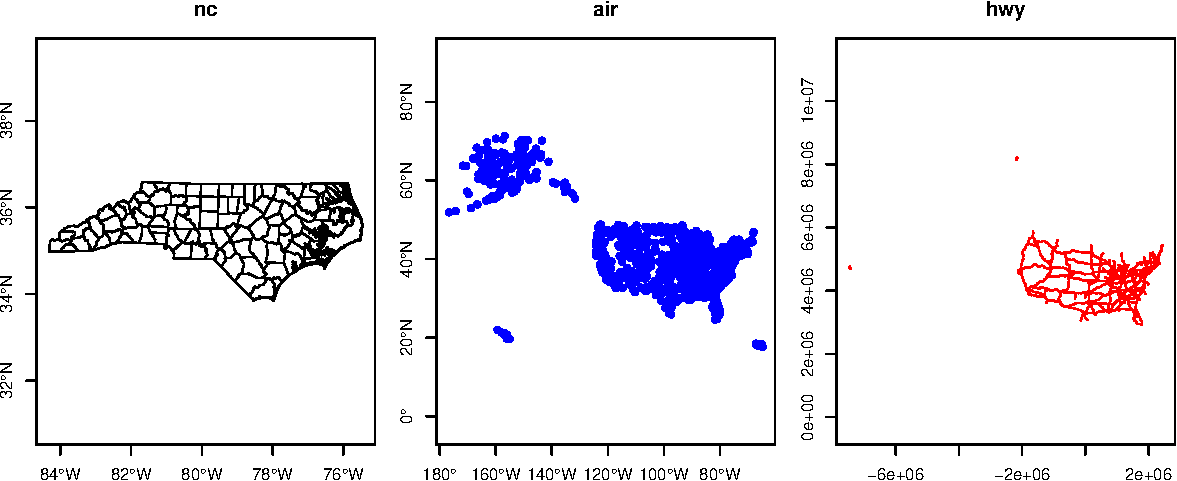
\includegraphics{Lec16_files/figure-beamer/unnamed-chunk-15-1} \end{center}

\end{frame}

\begin{frame}{UTM Zones}

\begin{center}
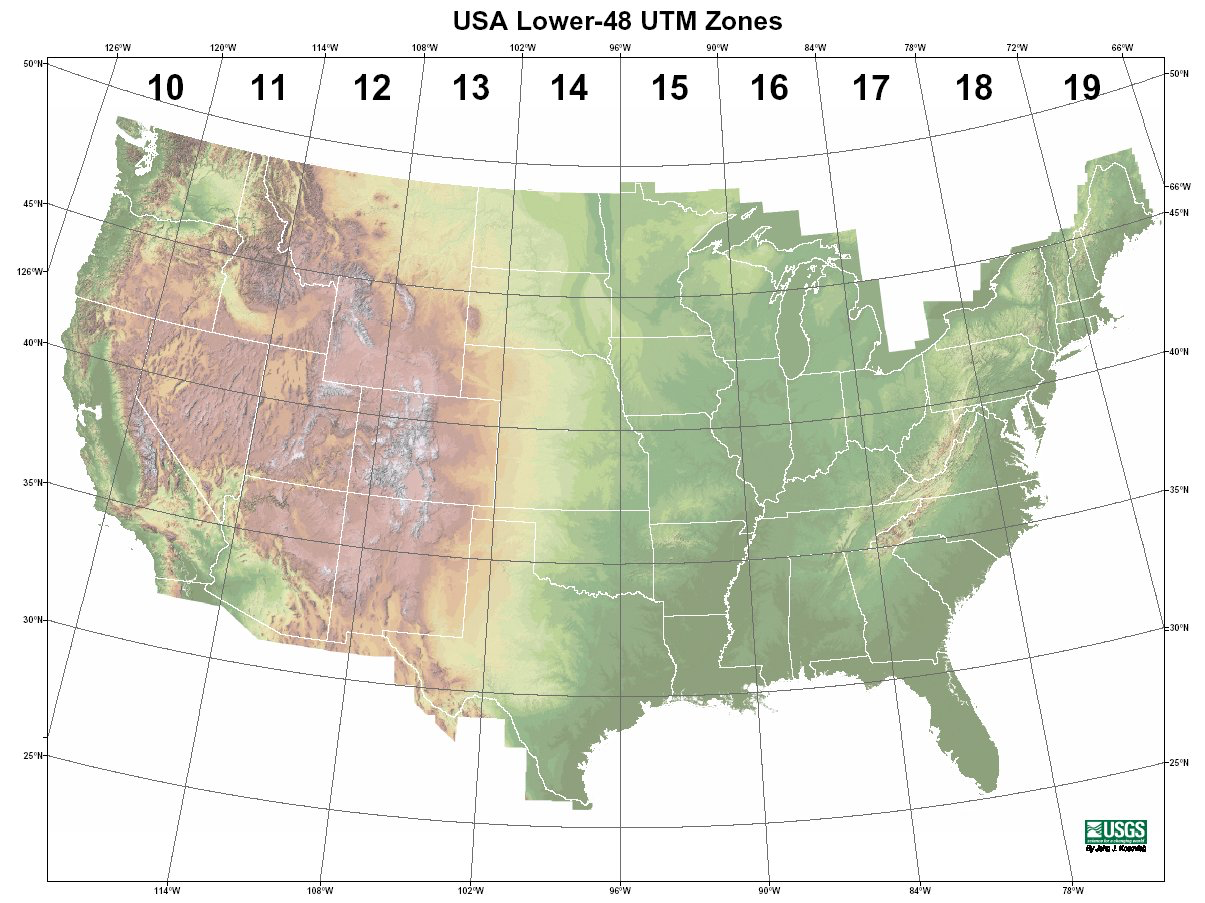
\includegraphics[width=0.9\textwidth]{figs/UTM_Zones.png}
\end{center}

\end{frame}

\begin{frame}[fragile]{Lat/Long}

\begin{Shaded}
\begin{Highlighting}[]
\NormalTok{nc_ll =}\StringTok{ }\NormalTok{nc}
\NormalTok{air_ll =}\StringTok{ }\NormalTok{air}
\NormalTok{hwy_ll =}\StringTok{ }\KeywordTok{st_transform}\NormalTok{(hwy, }\KeywordTok{st_crs}\NormalTok{(nc)}\OperatorTok{$}\NormalTok{proj4string)}
\end{Highlighting}
\end{Shaded}

\vspace{-5mm}

\begin{center}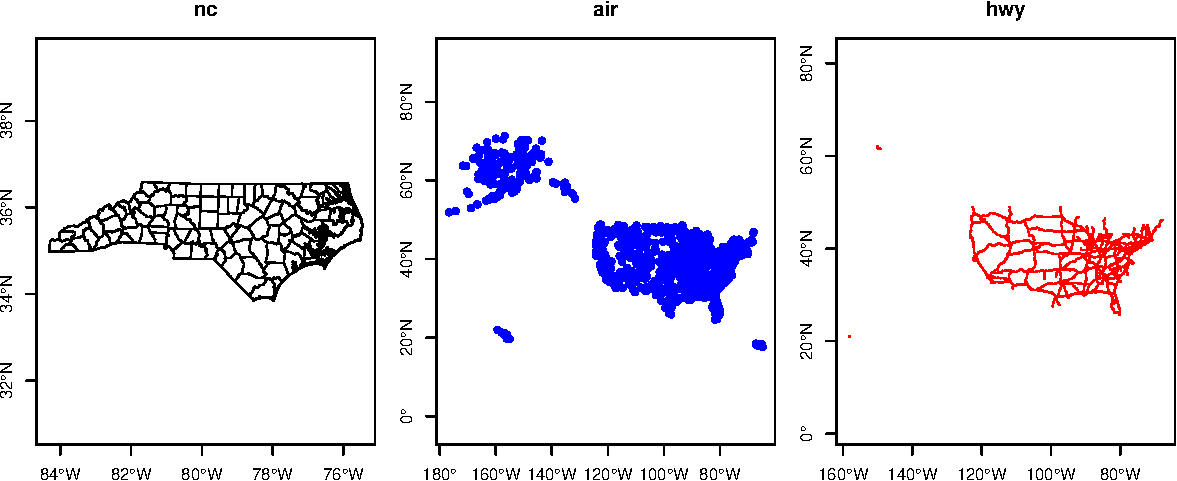
\includegraphics{Lec16_files/figure-beamer/unnamed-chunk-17-1} \end{center}

\end{frame}

\begin{frame}[fragile]{UTM}

\begin{Shaded}
\begin{Highlighting}[]
\NormalTok{nc_utm =}\StringTok{ }\KeywordTok{st_transform}\NormalTok{(nc, }\KeywordTok{st_crs}\NormalTok{(hwy)}\OperatorTok{$}\NormalTok{proj4string)}
\NormalTok{air_utm =}\StringTok{ }\KeywordTok{st_transform}\NormalTok{(air, }\KeywordTok{st_crs}\NormalTok{(hwy)}\OperatorTok{$}\NormalTok{proj4string)}
\NormalTok{hwy_utm =}\StringTok{ }\NormalTok{hwy}
\end{Highlighting}
\end{Shaded}

\vspace{-5mm}

\begin{center}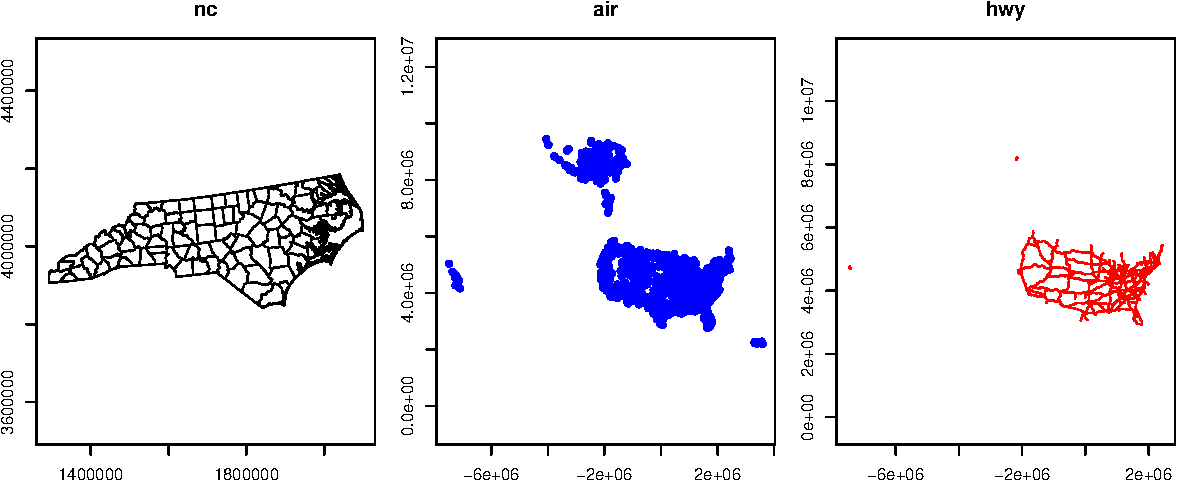
\includegraphics{Lec16_files/figure-beamer/unnamed-chunk-19-1} \end{center}

\end{frame}

\begin{frame}{Comparison}

\begin{center}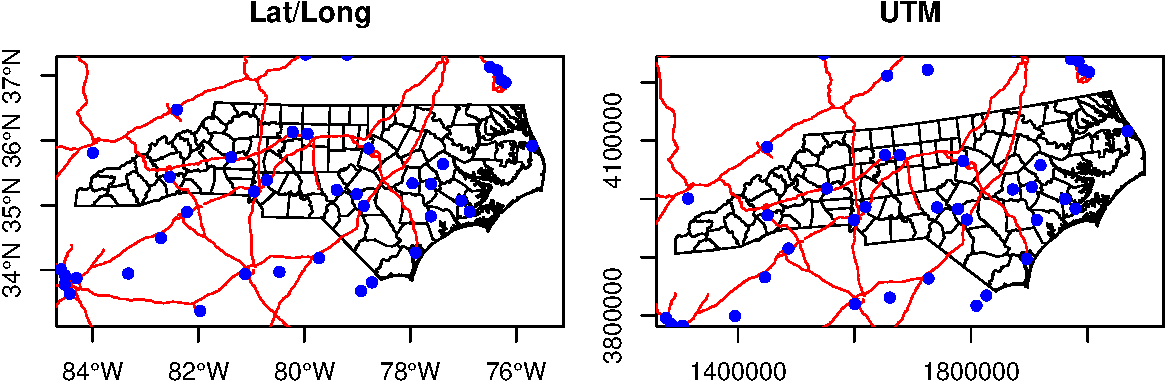
\includegraphics{Lec16_files/figure-beamer/unnamed-chunk-20-1} \end{center}

\end{frame}

\begin{frame}[fragile]{Subsetting vs.~dplyr}

\tinyoutput

\begin{Shaded}
\begin{Highlighting}[]
\NormalTok{sub =}\StringTok{ }\NormalTok{nc}\OperatorTok{$}\NormalTok{COUNTY }\OperatorTok\StringTok{ }\KeywordTok{c}\NormalTok{(}\StringTok{"Durham County"}\NormalTok{,}\StringTok{"Wake County"}\NormalTok{,}\StringTok{"Orange County"}\NormalTok{)}
\NormalTok{nc[sub,]}
\NormalTok{## Simple feature collection with 3 features and 8 fields}
\NormalTok{## geometry type:  MULTIPOLYGON}
\NormalTok{## dimension:      XY}
\NormalTok{## bbox:           xmin: -79.26453 ymin: 35.51905 xmax: -78.25503 ymax: 36.24385}
\NormalTok{## epsg (SRID):    4269}
\NormalTok{## proj4string:    +proj=longlat +datum=NAD83 +no_defs}
\NormalTok{##          AREA PERIMETER COUNTYP010 STATE        COUNTY  FIPS}
\NormalTok{## 29 0.10401267  1.297813       2074    NC Orange County 37135}
\NormalTok{## 30 0.07714111  1.287529       2075    NC Durham County 37063}
\NormalTok{## 37 0.22144442  2.140667       2106    NC   Wake County 37183}
\NormalTok{##    STATE_FIPS SQUARE_MIL                       geometry}
\NormalTok{## 29         37    401.465 MULTIPOLYGON(((-79.25563180...}
\NormalTok{## 30         37    297.841 MULTIPOLYGON(((-78.94843190...}
\NormalTok{## 37         37    857.610 MULTIPOLYGON(((-78.71263198...}
\end{Highlighting}
\end{Shaded}

\begin{Shaded}
\begin{Highlighting}[]
\KeywordTok{filter}\NormalTok{(nc, COUNTY }\OperatorTok\StringTok{ }\KeywordTok{c}\NormalTok{(}\StringTok{"Durham County"}\NormalTok{,}\StringTok{"Wake County"}\NormalTok{,}\StringTok{"Orange County"}\NormalTok{))}
\NormalTok{## Simple feature collection with 3 features and 8 fields}
\NormalTok{## geometry type:  MULTIPOLYGON}
\NormalTok{## dimension:      XY}
\NormalTok{## bbox:           xmin: -84.32186 ymin: 33.84175 xmax: -75.46003 ymax: 36.58815}
\NormalTok{## epsg (SRID):    4269}
\NormalTok{## proj4string:    +proj=longlat +datum=NAD83 +no_defs}
\NormalTok{##         AREA PERIMETER COUNTYP010 STATE        COUNTY  FIPS}
\NormalTok{## 1 0.10401267  1.297813       2074    NC Orange County 37135}
\NormalTok{## 2 0.07714111  1.287529       2075    NC Durham County 37063}
\NormalTok{## 3 0.22144442  2.140667       2106    NC   Wake County 37183}
\NormalTok{##   STATE_FIPS SQUARE_MIL                       geometry}
\NormalTok{## 1         37    401.465 MULTIPOLYGON(((-79.25563180...}
\NormalTok{## 2         37    297.841 MULTIPOLYGON(((-78.94843190...}
\NormalTok{## 3         37    857.610 MULTIPOLYGON(((-78.71263198...}
\end{Highlighting}
\end{Shaded}

\end{frame}

\begin{frame}[fragile,t]{Distance between NC counties}

\begin{Shaded}
\begin{Highlighting}[]
\NormalTok{counties =}\StringTok{ }\KeywordTok{c}\NormalTok{(}\StringTok{"Durham County"}\NormalTok{,}\StringTok{"Wake County"}\NormalTok{,}\StringTok{"Orange County"}\NormalTok{)}
\NormalTok{sub =}\StringTok{ }\NormalTok{nc}\OperatorTok{$}\NormalTok{COUNTY }\OperatorTok\StringTok{ }\NormalTok{counties}

\KeywordTok{st_distance}\NormalTok{(nc_ll[sub, ])}
\NormalTok{## Error in st_distance(nc_ll[sub, ]): st_distance for longitude/latitude data only available for POINT geometries}
\KeywordTok{st_distance}\NormalTok{(nc_utm[sub, ])}
\NormalTok{## Units: m}
\NormalTok{##          [,1] [,2]     [,3]}
\NormalTok{## [1,]    0.000    0 9906.327}
\NormalTok{## [2,]    0.000    0    0.000}
\NormalTok{## [3,] 9906.327    0    0.000}
\end{Highlighting}
\end{Shaded}

\end{frame}

\begin{frame}[fragile,t]{Distance between NC counties (centroids)}

\begin{Shaded}
\begin{Highlighting}[]
\NormalTok{nc_ll[sub, ] }\OperatorTok\StringTok{ }\KeywordTok{st_centroid}\NormalTok{() }\OperatorTok\StringTok{ }\KeywordTok{st_distance}\NormalTok{()}
\NormalTok{## Units: m}
\NormalTok{##          [,1]     [,2]     [,3]}
\NormalTok{## [1,]     0.00 22185.58 52031.22}
\NormalTok{## [2,] 22185.58     0.00 34076.78}
\NormalTok{## [3,] 52031.22 34076.78     0.00}

\NormalTok{nc_utm[sub, ] }\OperatorTok\StringTok{ }\KeywordTok{st_centroid}\NormalTok{() }\OperatorTok\StringTok{ }\KeywordTok{st_distance}\NormalTok{()}
\NormalTok{## Units: m}
\NormalTok{##          [,1]     [,2]     [,3]}
\NormalTok{## [1,]     0.00 22616.18 53050.15}
\NormalTok{## [2,] 22616.18     0.00 34751.60}
\NormalTok{## [3,] 53050.15 34751.60     0.00}
\end{Highlighting}
\end{Shaded}

\end{frame}

\begin{frame}[fragile,t]{Distance to the closest airport from each
county?}

\begin{Shaded}
\begin{Highlighting}[]
\NormalTok{d =}\StringTok{ }\KeywordTok{st_distance}\NormalTok{(air_utm, nc_utm[sub,]) }
\NormalTok{d[}\DecValTok{1}\OperatorTok{:}\DecValTok{5}\NormalTok{,]}
\NormalTok{## Units: m}
\NormalTok{##           [,1]      [,2]      [,3]}
\NormalTok{## [1,]  846916.0  837771.1  836234.3}
\NormalTok{## [2,] 3122697.5 3146840.3 3172522.0}
\NormalTok{## [3,] 3556664.1 3584394.6 3592972.9}
\NormalTok{## [4,] 3514296.0 3540264.5 3545184.1}
\NormalTok{## [5,]  952881.7  954495.9  921201.2}
\end{Highlighting}
\end{Shaded}

\begin{Shaded}
\begin{Highlighting}[]
\NormalTok{nearest_airport =}\StringTok{ }\KeywordTok{apply}\NormalTok{(d, }\DecValTok{2}\NormalTok{, which.min) }
\NormalTok{air }\OperatorTok\StringTok{ }\KeywordTok{slice}\NormalTok{(nearest_airport) }\OperatorTok\StringTok{ }\NormalTok{.}\OperatorTok{$}\NormalTok{AIRPT_NAME}
\NormalTok{## [1] "RALEIGH-DURHAM INTERNATIONAL AIRPORT"}
\NormalTok{## [2] "RALEIGH-DURHAM INTERNATIONAL AIRPORT"}
\NormalTok{## [3] "RALEIGH-DURHAM INTERNATIONAL AIRPORT"}
\end{Highlighting}
\end{Shaded}

\end{frame}

\section{Geometry Predicates}\label{geometry-predicates}

\begin{frame}[t]{DE-9IM}

\begin{center}
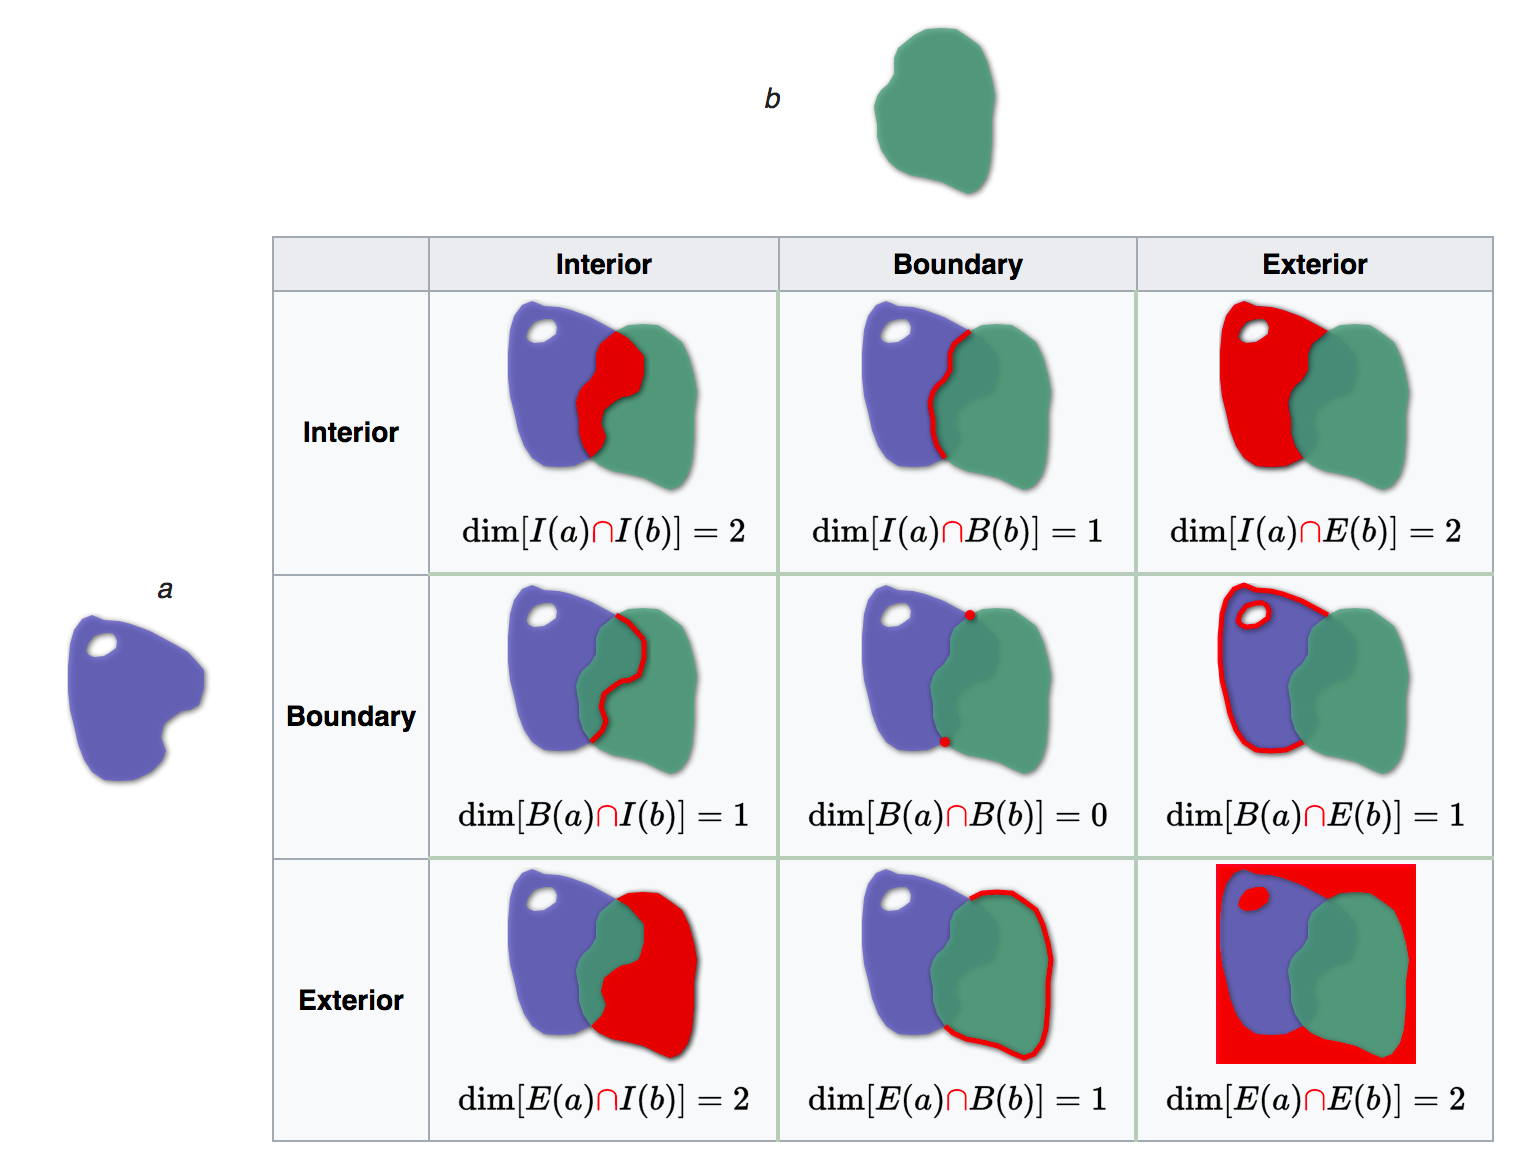
\includegraphics[width=0.95\textwidth]{figs/de_9im.png}
\end{center}

\end{frame}

\begin{frame}{Spatial predicates}

\begin{center}
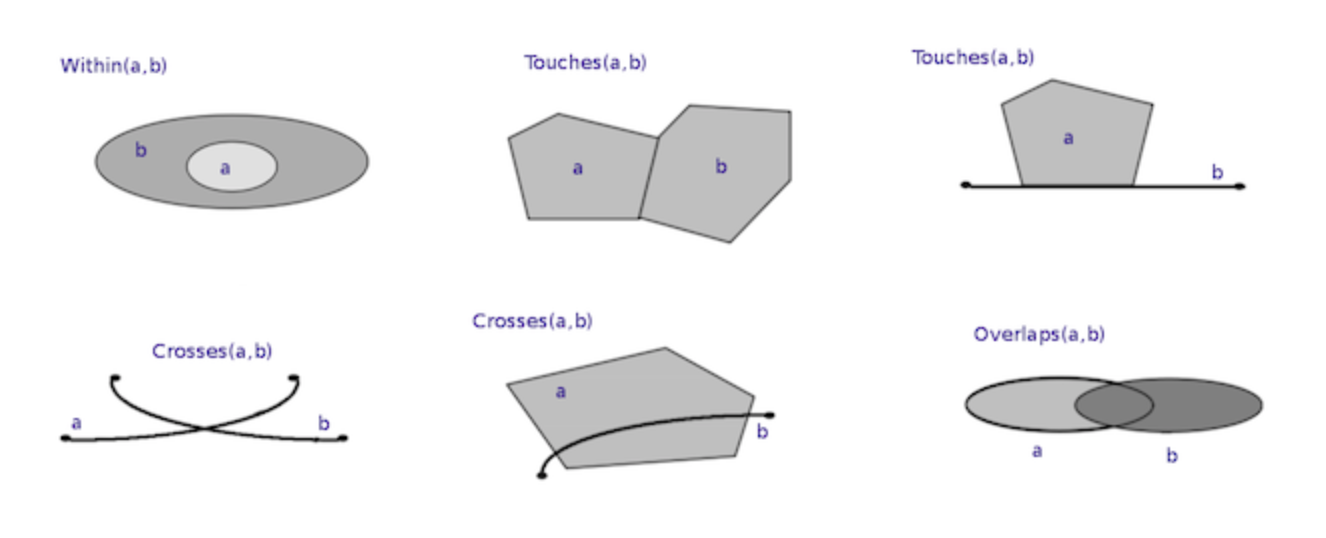
\includegraphics[width=0.75\textwidth]{figs/predicates.png}
\end{center}

\footnotesize

\hspace*{-4pt}\makebox[\linewidth][c]{
\begin{tabular}{lll}

st\_within(a,b) & & st\_touches(a,b) \\

$\begin{bmatrix} T & * & F \\ * & * & F \\ * & * & * \end{bmatrix}$ & &
$\begin{bmatrix} F & T & * \\ * & * & * \\ * & * & * \end{bmatrix} \cup 
\begin{bmatrix} F & * & * \\ T & * & * \\ * & * & * \end{bmatrix} \cup 
\begin{bmatrix} F & * & * \\ * & T & * \\ * & * & * \end{bmatrix}$ \\

\\

st\_crosses(a,b) & & st\_overlaps(a,b) ($\text{dim}(a) = \text{dim}(b)$) \\

$\overset{\text{If dim}(a) < \text{dim}(b)}{\begin{bmatrix} T & * & T \\ * & * & * \\ * & * & * \end{bmatrix}} ~~~
\overset{\text{If dim}(a) > \text{dim}(b)}{\begin{bmatrix} T & * & * \\ * & * & * \\ T & * & * \end{bmatrix}} ~~~
\overset{\text{If dim}(any) = 1}{\begin{bmatrix} 0 & * & * \\ * & * & * \\ * & * & * \end{bmatrix}}$ & &
$\overset{\text{If dim} \in \{0,2\}}{\begin{bmatrix} T & * & T \\ * & * & * \\ T & * & * \end{bmatrix}} ,~
\overset{\text{If dim} = 1}{\begin{bmatrix} 1 & * & T \\ * & * & * \\ T & * & * \end{bmatrix}}$ \\
\end{tabular}
}

\end{frame}

\begin{frame}[fragile]{Sparse vs Full Results}

\begin{Shaded}
\begin{Highlighting}[]
\KeywordTok{st_intersects}\NormalTok{(nc[}\DecValTok{20}\OperatorTok{:}\DecValTok{30}\NormalTok{,], air) }\OperatorTok\StringTok{ }\KeywordTok{str}\NormalTok{()}
\NormalTok{## List of 11}
\NormalTok{##  $ : int(0) }
\NormalTok{##  $ : int(0) }
\NormalTok{##  $ : int(0) }
\NormalTok{##  $ : int(0) }
\NormalTok{##  $ : int(0) }
\NormalTok{##  $ : int 268}
\NormalTok{##  $ : int 717}
\NormalTok{##  $ : int(0) }
\NormalTok{##  $ : int(0) }
\NormalTok{##  $ : int(0) }
\NormalTok{##  $ : int(0)}
\end{Highlighting}
\end{Shaded}

\begin{Shaded}
\begin{Highlighting}[]
\KeywordTok{st_intersects}\NormalTok{(nc, air, }\DataTypeTok{sparse=}\OtherTok{FALSE}\NormalTok{) }\OperatorTok\StringTok{ }\KeywordTok{str}\NormalTok{()}
\NormalTok{##  logi [1:100, 1:940] FALSE FALSE FALSE FALSE FALSE FALSE ...}
\end{Highlighting}
\end{Shaded}

\end{frame}

\begin{frame}[fragile,t]{Which counties have airports?}

\begin{Shaded}
\begin{Highlighting}[]
\NormalTok{nc_air =}\StringTok{ }\KeywordTok{st_intersects}\NormalTok{(nc, air)}
\NormalTok{has_air =}\StringTok{ }\KeywordTok{map_lgl}\NormalTok{(nc_air, }\OperatorTok{~}\StringTok{ }\KeywordTok{length}\NormalTok{(.) }\OperatorTok{>}\StringTok{ }\DecValTok{0}\NormalTok{)}
\NormalTok{nc }\OperatorTok\StringTok{ }\KeywordTok{slice}\NormalTok{(}\KeywordTok{which}\NormalTok{(has_air)) }\OperatorTok\StringTok{ }\NormalTok{.}\OperatorTok{$}\NormalTok{COUNTY}
\NormalTok{##  [1] "Forsyth County"     "Guilford County"    "Dare County"       }
\NormalTok{##  [4] "Wake County"        "Pitt County"        "Catawba County"    }
\NormalTok{##  [7] "Buncombe County"    "Wayne County"       "Mecklenburg County"}
\NormalTok{## [10] "Moore County"       "Cabarrus County"    "Lenoir County"     }
\NormalTok{## [13] "Craven County"      "Cumberland County"  "Onslow County"     }
\NormalTok{## [16] "New Hanover County"}
\end{Highlighting}
\end{Shaded}

\begin{Shaded}
\begin{Highlighting}[]
\NormalTok{air_in_nc =}\StringTok{ }\NormalTok{nc_air }\OperatorTok\StringTok{ }\KeywordTok{unlist}\NormalTok{() }\OperatorTok\StringTok{ }\KeywordTok{unique}\NormalTok{()}
\NormalTok{air }\OperatorTok\StringTok{ }\KeywordTok{slice}\NormalTok{(air_in_nc) }\OperatorTok\StringTok{ }\NormalTok{.}\OperatorTok{$}\NormalTok{AIRPT_NAME}
\NormalTok{##  [1] "SMITH REYNOLDS AIRPORT"                                  }
\NormalTok{##  [2] "PIEDMONT TRIAD INTERNATIONAL AIRPORT"                    }
\NormalTok{##  [3] "DARE COUNTY REGIONAL AIRPORT"                            }
\NormalTok{##  [4] "RALEIGH-DURHAM INTERNATIONAL AIRPORT"                    }
\NormalTok{##  [5] "PITT-GREENVILLE AIRPORT"                                 }
\NormalTok{##  [6] "HICKORY REGIONAL AIRPORT"                                }
\NormalTok{##  [7] "ASHEVILLE REGIONAL AIRPORT"                              }
\NormalTok{##  [8] "SEYMOUR JOHNSON AIR FORCE BASE"                          }
\NormalTok{##  [9] "CHARLOTTE/DOUGLAS INTERNATIONAL AIRPORT"                 }
\NormalTok{## [10] "MOORE COUNTY AIRPORT"                                    }
\NormalTok{## [11] "CONCORD REGIONAL AIRPORT"                                }
\NormalTok{## [12] "KINSTON REGIONAL JETPORT AT STALLINGS FIELD"             }
\NormalTok{## [13] "CHERRY POINT MARINE CORPS AIR STATION /CUNNINGHAM FIELD/"}
\NormalTok{## [14] "COASTAL CAROLINA REGIONAL AIRPORT"                       }
\NormalTok{## [15] "POPE AIR FORCE BASE"                                     }
\NormalTok{## [16] "FAYETTEVILLE REGIONAL/GRANNIS FIELD"                     }
\NormalTok{## [17] "ALBERT J ELLIS AIRPORT"                                  }
\NormalTok{## [18] "WILMINGTON INTERNATIONAL AIRPORT"}
\end{Highlighting}
\end{Shaded}

\end{frame}

\begin{frame}[fragile,t]{}

\begin{Shaded}
\begin{Highlighting}[]
\KeywordTok{plot}\NormalTok{(}\KeywordTok{st_geometry}\NormalTok{(nc))}
\KeywordTok{plot}\NormalTok{(}\KeywordTok{st_geometry}\NormalTok{(nc[has_air,]), }\DataTypeTok{add=}\OtherTok{TRUE}\NormalTok{, }\DataTypeTok{col=}\StringTok{"lightblue"}\NormalTok{)}
\KeywordTok{plot}\NormalTok{(}\KeywordTok{st_geometry}\NormalTok{(air[air_in_nc,]), }\DataTypeTok{add=}\OtherTok{TRUE}\NormalTok{, }\DataTypeTok{pch=}\DecValTok{16}\NormalTok{, }\DataTypeTok{col=}\StringTok{"blue"}\NormalTok{)}
\end{Highlighting}
\end{Shaded}

\begin{center}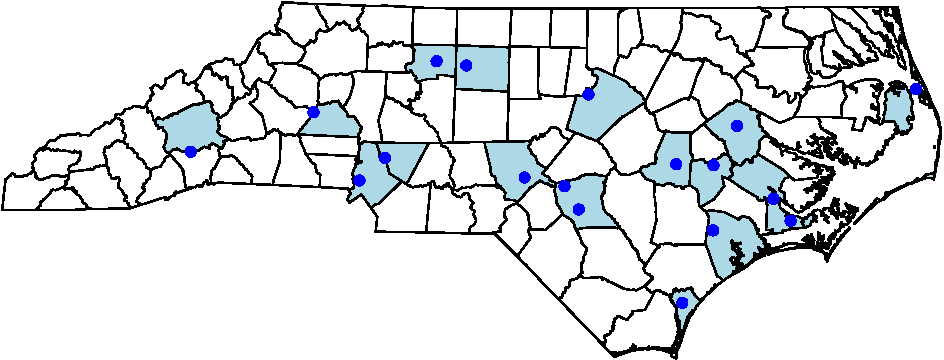
\includegraphics{Lec16_files/figure-beamer/unnamed-chunk-31-1} \end{center}

\end{frame}

\begin{frame}[fragile,t]{Adjacency matrix of counties}

\begin{Shaded}
\begin{Highlighting}[]
\NormalTok{nc =}\StringTok{ }\NormalTok{nc[}\KeywordTok{order}\NormalTok{(nc}\OperatorTok{$}\NormalTok{COUNTY),]}
\NormalTok{adj =}\StringTok{ }\KeywordTok{st_touches}\NormalTok{(nc, }\DataTypeTok{sparse=}\OtherTok{FALSE}\NormalTok{)}

\KeywordTok{str}\NormalTok{(adj)}
\NormalTok{##  logi [1:100, 1:100] FALSE FALSE FALSE FALSE FALSE FALSE ...}

\NormalTok{durham =}\StringTok{ }\KeywordTok{which}\NormalTok{(nc}\OperatorTok{$}\NormalTok{COUNTY }\OperatorTok{==}\StringTok{ "Durham County"}\NormalTok{)}
\NormalTok{nc }\OperatorTok\StringTok{ }\KeywordTok{slice}\NormalTok{(}\KeywordTok{which}\NormalTok{(adj[durham,])) }\OperatorTok\StringTok{ }\NormalTok{.}\OperatorTok{$}\NormalTok{COUNTY}
\NormalTok{## [1] "Chatham County"   "Granville County" "Orange County"   }
\NormalTok{## [4] "Person County"    "Wake County"}
\end{Highlighting}
\end{Shaded}

\end{frame}

\begin{frame}[fragile]{}

\begin{Shaded}
\begin{Highlighting}[]
\KeywordTok{library}\NormalTok{(corrplot)}
\KeywordTok{rownames}\NormalTok{(adj) =}\StringTok{ }\KeywordTok{str_replace}\NormalTok{(nc}\OperatorTok{$}\NormalTok{COUNTY, }\StringTok{" County"}\NormalTok{, }\StringTok{""}\NormalTok{)}
\KeywordTok{colnames}\NormalTok{(adj) =}\StringTok{ }\KeywordTok{str_replace}\NormalTok{(nc}\OperatorTok{$}\NormalTok{COUNTY, }\StringTok{" County"}\NormalTok{, }\StringTok{""}\NormalTok{)}
\KeywordTok{corrplot}\NormalTok{(adj[}\DecValTok{1}\OperatorTok{:}\DecValTok{20}\NormalTok{,}\DecValTok{1}\OperatorTok{:}\DecValTok{20}\NormalTok{],}\DataTypeTok{method=}\StringTok{"color"}\NormalTok{,}\DataTypeTok{type=}\StringTok{"full"}\NormalTok{,}\DataTypeTok{tl.col=}\StringTok{"black"}\NormalTok{,}\DataTypeTok{cl.pos =} \StringTok{"n"}\NormalTok{)}
\end{Highlighting}
\end{Shaded}

\begin{center}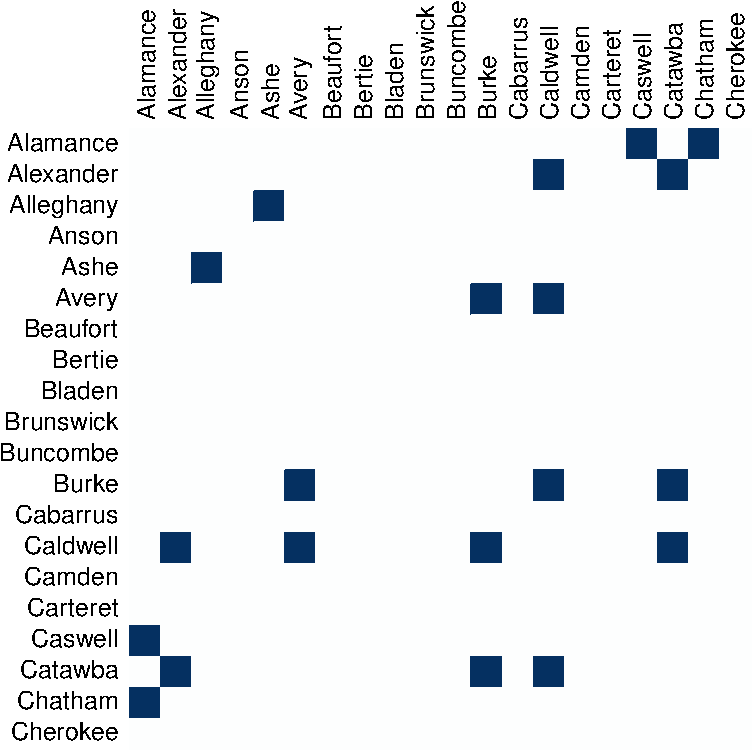
\includegraphics{Lec16_files/figure-beamer/unnamed-chunk-33-1} \end{center}

\end{frame}

\begin{frame}[fragile]{Which counties have the most neighbors?}

\begin{Shaded}
\begin{Highlighting}[]
\NormalTok{most_neighbors =}\StringTok{ }\KeywordTok{rowSums}\NormalTok{(adj)}\OperatorTok{==}\KeywordTok{max}\NormalTok{(}\KeywordTok{rowSums}\NormalTok{(adj)) }
\KeywordTok{plot}\NormalTok{(}\KeywordTok{st_geometry}\NormalTok{(nc))}
\KeywordTok{plot}\NormalTok{(}\KeywordTok{st_geometry}\NormalTok{(nc[most_neighbors,]),}\DataTypeTok{add=}\OtherTok{TRUE}\NormalTok{,}\DataTypeTok{col=}\StringTok{"lightblue"}\NormalTok{)}
\end{Highlighting}
\end{Shaded}

\begin{center}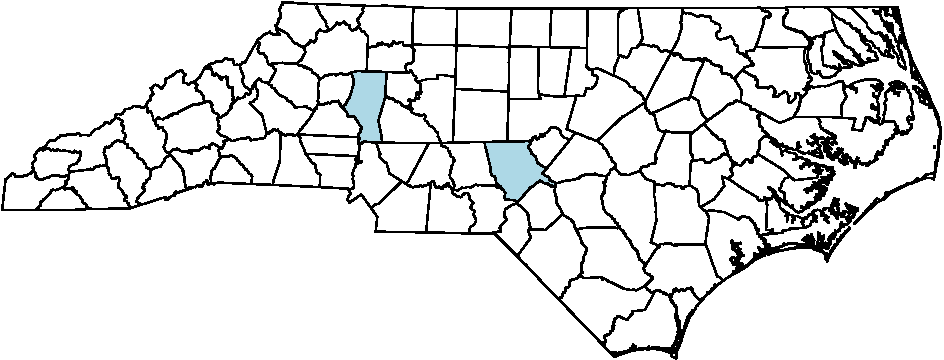
\includegraphics{Lec16_files/figure-beamer/unnamed-chunk-34-1} \end{center}

\begin{Shaded}
\begin{Highlighting}[]
\NormalTok{nc}\OperatorTok{$}\NormalTok{COUNTY[most_neighbors]}
\NormalTok{## [1] "Iredell County" "Moore County"}
\end{Highlighting}
\end{Shaded}

\end{frame}

\begin{frame}[fragile]{Which counties have the least neighbors?}

\begin{Shaded}
\begin{Highlighting}[]
\NormalTok{least_neighbors =}\StringTok{ }\KeywordTok{rowSums}\NormalTok{(adj)}\OperatorTok{==}\KeywordTok{min}\NormalTok{(}\KeywordTok{rowSums}\NormalTok{(adj)) }
\KeywordTok{plot}\NormalTok{(}\KeywordTok{st_geometry}\NormalTok{(nc))}
\KeywordTok{plot}\NormalTok{(}\KeywordTok{st_geometry}\NormalTok{(nc[least_neighbors,]),}\DataTypeTok{add=}\OtherTok{TRUE}\NormalTok{,}\DataTypeTok{col=}\StringTok{"lightblue"}\NormalTok{)}
\end{Highlighting}
\end{Shaded}

\begin{center}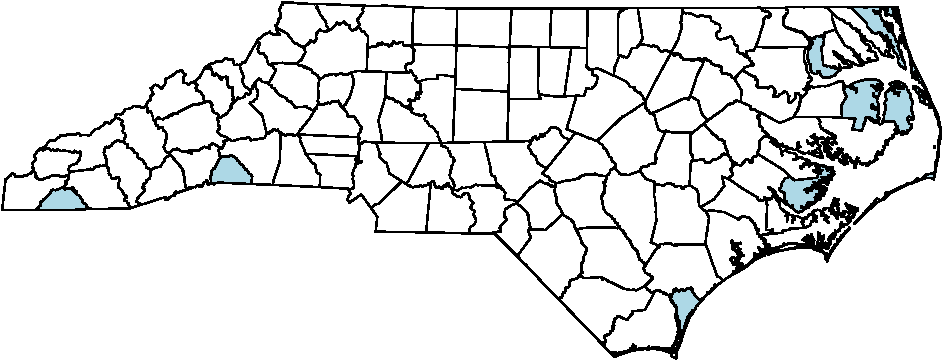
\includegraphics{Lec16_files/figure-beamer/unnamed-chunk-35-1} \end{center}

\begin{Shaded}
\begin{Highlighting}[]
\NormalTok{nc}\OperatorTok{$}\NormalTok{COUNTY[least_neighbors]}
\NormalTok{## [1] "Chowan County"      "Clay County"        "Currituck County"  }
\NormalTok{## [4] "Dare County"        "New Hanover County" "Pamlico County"    }
\NormalTok{## [7] "Polk County"        "Tyrrell County"}
\end{Highlighting}
\end{Shaded}

\end{frame}

\end{document}
